%======================================================================
\section{El escenario único de Homem-de-Mello et al.\ (F9)}\label{sec:rozas}
%======================================================================
En la reunión del 22 de octubre H.~Rozas propuso dos vías: linealizar el reactor (V2, base de
N1/N2) y \emph{aprender un escenario único} que, puesto en el MPC determinista, reproduzca la
decisión estocástica (V6), con el artículo de Homem-de-Mello, Valencia, Lagos y
Lagos~\cite{homem2026}. La proposición~\ref{prop:margen}(b) mostró que para las \emph{cotas}
(cuantil, CVaR, Wilks) ese escenario existe, es físico y es explícito. Esta sección comprueba,
con la metodología del propio artículo, si el SMDFR cumple sus condiciones y qué pasa con las
formulaciones que no son cotas: la pérdida esperada y las fallas parciales dentro del horizonte.

\subsection{El teorema y sus condiciones}
El artículo estudia programas de dos etapas con \emph{recurso fijo y costos fijos} (FRFC):
\[
\min_{z\in Z}\ f(z)+\mathbb E\big[Q(z,\xi)\big],\qquad
Q(z,\xi)=\min\{q^\top y:\ Wy=h-Tz,\ y\ge0\},\quad \xi=(h,T),
\]
con $W$ y $q$ deterministas. Su teorema~1 afirma que, si el conjunto dual
$U=\{u:\ W^\top u\le q\}$ es no vacío y acotado (supuesto~2) y además (i) $T$ es determinista o
(ii) $T$ es aleatoria y cumple su lema~1 ($n<m$; o $n=m$ con $0\in\operatorname{int}U$; o $n=m$,
$0$ punto extremo de $U$ y $-T^\top U$ dentro de un ortante), entonces el escenario
$\xi^*=(T^*z^*,T^*)$ reproduce la solución estocástica $z^*$, y es la única si el problema de un
escenario tiene solución única (supuesto~3). La idea de la demostración: con $h^*=T^*z^*$ el
lado derecho de la segunda etapa se anula en $z^*$, todos los duales son óptimos y el
subdiferencial de $Q(\cdot,\xi^*)$ es el conjunto entero $-T^{*\top}U$, que contiene al
subgradiente esperado. Como $\xi^*$ se construye con $z^*$, el teorema no ahorra cómputo en una
consulta aislada. Su uso práctico es el caso \emph{contextual}: aprender un pronóstico
$\Phi(\theta,x)\approx\xi^*_x$ que dependa del estado $x$, entrenado por la calidad de la
decisión (algoritmo~1 del artículo: pronosticar, planificar, medir el costo realizado y
ajustar $\theta$ con Nelder--Mead).

En el SMDFR la primera etapa es el plan $u\in\mathbb R^{26}$ del QP de N2 (caja $[0,40]$~kg/s,
rampa dura de 5~kg/s, $R=0.1$) y $f$ es su costo. Se prueban tres segundas etapas
(tabla~\ref{tab:f9-condiciones}).

\begin{table}[H]\centering\small
\caption{Las tres segundas etapas y las condiciones del teorema~1. $G$ es la matriz de
sensibilidad de la PCT predicha al caudal ($\hat y=y_0+Gu$).}
\label{tab:f9-condiciones}
\begin{tabular}{@{}>{\raggedright\arraybackslash}p{3.5cm}>{\raggedright\arraybackslash}p{3.9cm}>{\raggedright\arraybackslash}p{1.9cm}>{\raggedright\arraybackslash}p{4.3cm}@{}}
\toprule
Segunda etapa & Incertidumbre & Caso & ¿Cumple?\\
\midrule
P1: pérdida esperada $\rho\sum_k(\hat y_k+d+\Delta T(D)-1220)_+$ & duración $D$ de una falla total que empieza ahora & (i): $T=-G$ fija & sí\\
P2: fallas parciales dentro del horizonte & inicio $j$, severidad $\eta$, duración $D$; la planta recibe $\eta u$ & (ii): $T$ aleatoria & como está implementada (una fila por escenario, $m=1<n=26$): \textbf{no}; escrita por paso ($m=n=26$): sí, lema~1~(iii), porque todos los $G_{ki}<0$\\
P3: seguimiento en $L_1$ con error de pronóstico de fuga & $\delta L\sim\mathcal N(0,\Sigma_L)$ (Kalman, F5b.0) & (i) & sí\\
\bottomrule
\end{tabular}
\end{table}

\noindent El supuesto~3 merece una nota. Sin supresión de movimiento,
$\lambda_{\min}(G^\top G)\approx1.6\cdot10^{-6}$: el QP es casi singular y planes muy distintos
dan casi el mismo costo. Con $R=0.1$ (sección~\ref{sec:supresion}),
$\lambda_{\min}(G^\top G+RD^\top D)\approx2.2\cdot10^{-3}$ en todas las consultas. \textbf{La
unicidad que pide el teorema la da la supresión de movimiento.}

\subsection{Experimento}
Se capturaron las consultas de 50 lazos cerrados (familia DET acelerada, $\mu\times10^4$,
40~kg/s, N2 con la pérdida esperada $\rho=1000$, $R=0.1$, fallas del DET): una de cada seis,
4050 consultas, de las cuales 1050 también para P2 y P3. En cada una se reconstruye el QP del
lazo (reproduce su decisión con error $\le0.011$~kg/s) y se hacen las comprobaciones del
artículo: E1, los supuestos; E2, el teorema~1 en forma constructiva; E3, el problema
bilevel~(38)--(39) del artículo resuelto sin derivadas, pero restringido a escenarios
\emph{físicos}; E4, el caso contextual; E5, el lazo cerrado. Los QP se resuelven con Clarabel
con tolerancias de $10^{-10}$: con tolerancias estándar ($10^{-8}$) las diferencias que se miden
quedan dentro del ruido del solver. Código: \code{julia/F9Rozas.jl}, \code{julia/f9\_rozas.jl};
resultados: \code{results/f9\_rozas/summary.md}. Son 50 lazos y unos 3~millones de QP, en
51~min con 20 procesos en Olab.

\subsection{E2: el escenario del teorema existe, pero no es físico}
Se resuelve el SAA (200 cuantiles de $D$), se construye $\xi^*$ con su solución y se resuelve el
problema de un escenario. La tabla~\ref{tab:f9-teorema} confirma el teorema en las tres
formulaciones, incluida la P2 implementada, que queda fuera del lema~1. Allí también existe un
escenario: el teorema encierra todo el conjunto $\mathbb E[-T^\top U]$, pero la optimalidad de
$z^*$ sólo necesita su subgradiente, y basta una fila $a^*=g/\rho$ con el pliegue en $z^*$.

\begin{table}[H]\centering\small
\caption{Teorema~1 constructivo: distancia entre el plan del escenario $\xi^*$ y el plan SAA
(4050 consultas; P2 y P3 en 1050).}
\label{tab:f9-teorema}
\begin{tabular}{@{}lllll@{}}
\toprule
Formulación & Caso & $\|u_{\xi^*}-u_{\rm SAA}\|_\infty$ mediana & máx. & $|\Delta J|$ máx.\\
\midrule
P1, $\rho=100$ & (i) & $7.9\cdot10^{-6}$ & $8.8\cdot10^{-4}$ & $3.6\cdot10^{-5}$\\
P1, $\rho=1000$ & (i) & $1.4\cdot10^{-5}$ & $3.6\cdot10^{-4}$ & $2.4\cdot10^{-5}$\\
P2 implementada, $\rho=1000$ & fuera del lema~1 & $1.8\cdot10^{-5}$ & $0.017$ & $2.4\cdot10^{-4}$\\
P2 por paso, $\rho=1000$ & (ii), lema~1~(iii) & $1.7\cdot10^{-5}$ & $0.022$ & $8.1\cdot10^{-5}$\\
P3 & (i) & $5.2\cdot10^{-5}$ & $5.1\cdot10^{-4}$ & $3.2\cdot10^{-7}$\\
\bottomrule
\end{tabular}
\end{table}

\noindent Pero $\xi^*$ no es un evento posible. En P1 es un margen \emph{distinto en cada paso}
(dispersión mediana de 2.4~K entre pasos), mientras que el calentamiento $\Delta T(D)$ de una
falla es el mismo para todos los pasos. En P3, traducido a error de pronóstico de la fuga, está a
$\sim10^5$ desviaciones estándar del pronóstico. El artículo lo anticipa: el escenario óptimo
puede estar fuera del soporte. La pregunta práctica es entonces si basta un escenario
\emph{físico}.

\subsection{E3: un escenario físico casi basta, el pronóstico puntual no}
El bilevel~(38)--(39) busca el escenario que minimiza el costo SAA de la decisión que induce. Se
resolvió como en el artículo, sin derivadas (malla de 301 márgenes y sección áurea), restringido
a una sola falla total de duración $\hat D$ (P1) o a una falla $(\hat j,\hat\eta,\hat D)$ (P2).
La figura~\ref{fig:f9-theorem} y la tabla~\ref{tab:f9-bilevel} comparan ese escenario con el del
teorema y con el pronóstico puntual, la duración media $\mathbb E[D]\approx46$~s.

\begin{figure}[H]\centering
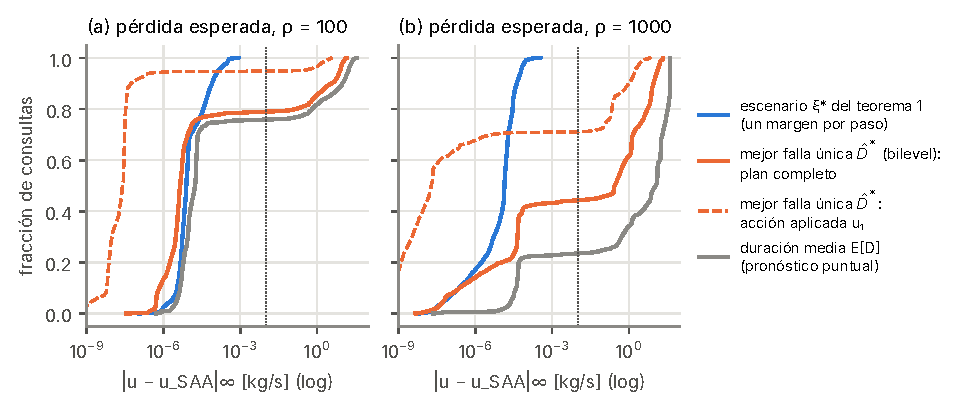
\includegraphics[width=\linewidth]{figures/fig_f9_theorem.pdf}
\caption{Distribución, sobre 4050 consultas, de la distancia al plan SAA. Azul: el escenario
del teorema~1, siempre dentro de la tolerancia del solver. Naranja: la mejor falla única
(línea continua, plan completo; discontinua, acción aplicada $u_1$). Gris: la duración media.
Línea punteada: 0.01~kg/s.}
\label{fig:f9-theorem}
\end{figure}

\begin{table}[H]\centering\footnotesize\setlength{\tabcolsep}{3.5pt}
\caption{Escenarios únicos físicos (P1) y su pérdida respecto del SAA, en fracción del valor de
la solución estocástica (VSS $=J_{\mathbb E}$(N2 sin riesgo)$-J_{\mathbb E}$(SAA), agregado
sobre 4050 consultas; costo esperado con 1000 cuantiles de $D$).}
\label{tab:f9-bilevel}
\begin{tabular}{@{}lcccc@{}}
\toprule
& \multicolumn{2}{c}{$\rho=100$} & \multicolumn{2}{c}{$\rho=1000$}\\
\cmidrule(lr){2-3}\cmidrule(lr){4-5}
Escenario único & pérdida/VSS & $\|\Delta u\|_\infty<0.01$ & pérdida/VSS & $\|\Delta u\|_\infty<0.01$\\
\midrule
Mejor duración $\hat D^*$ (bilevel) & 0.063 & 79\,\% & 0.005 & 44\,\%\\
Cuantil 0.98 de $D$ & 35 & 60\,\% & 0.13 & 42\,\%\\
Duración media o mediana (pronóstico puntual) & 1 & 76\,\% & 1 & 23\,\%\\
\bottomrule
\end{tabular}
\end{table}

\begin{enumerate}
  \item \textbf{El pronóstico puntual pierde todo el VSS.} Con $\mathbb E[D]\approx46$~s el
        calentamiento es de unos 12~K y la cota nunca se activa: la decisión es la de N2 sin
        riesgo. Es el mensaje central del artículo: el escenario que mejor decide no es el más
        probable.
  \item \textbf{Una falla única bien elegida recupera el 94\,\% ($\rho=100$) y el 99.5\,\%
        ($\rho=1000$) del VSS.} Su duración mediana es de 170--190~s, unas cuatro veces la media:
        está en la cola de la distribución. La acción que se aplica, $u_1$, coincide con la del
        SAA (a menos de 0.01~kg/s) en el 95\,\% ($\rho=100$) y el 71\,\% ($\rho=1000$) de las
        consultas; las demás diferencias están en la cola del plan, que el MPC reoptimiza en la
        consulta siguiente. En el 10--16\,\% de las consultas el mejor escenario es «ninguna
        falla»: allí la capa de riesgo no cambia la decisión.
  \item \textbf{Un cuantil fijo no reemplaza al escenario óptimo.} El cuantil 0.98 es muy
        conservador con $\rho=100$ (pierde 35 veces el VSS) y razonable con $\rho=1000$. Para la
        pérdida esperada, a diferencia de las cotas, el escenario depende de $\rho$ y del estado.
  \item \textbf{Fallas parciales y pronóstico de fuga: no hay nada que recuperar.} En P2 la falla
        física única pierde el 60\,\% del VSS, pero el VSS medio es $0.02$ (frente a 280 en P1): el
        riesgo dentro del horizonte es despreciable, como en la sección~\ref{sec:riesgo-parciales}.
        En P3 el equivalente cierto ($\delta L=0$) ya es óptimo: el error de pronóstico mueve la
        PCT predicha menos de 0.005~K.
\end{enumerate}

\paragraph{Costo computacional.} El artículo observa que la búsqueda del escenario crece
linealmente con el número de muestras $N$ y el SAA como LP, exponencialmente. Aquí
(figura~\ref{fig:f9-learning}a) el SAA es un QP disperso y crece aproximadamente lineal (de
0.02~s con $N=10$ a 8.6~s con $N=4000$), y la búsqueda cuesta unos 2.7~s casi constantes (301 QP
de un escenario). El SAA es más rápido hasta $N\approx2000$; con los 40 cuantiles del lazo
(0.06~s) no hay ventaja computacional que ganar.

\subsection{E4: el caso contextual}\label{sec:rozas-contextual}
Ésta es la propuesta de Rozas propiamente dicha: aprender, fuera de línea, un pronóstico del
escenario en función del contexto, $\hat\delta=\Phi(\theta,x)$, para que en línea sólo se resuelva
el MPC determinista con ese escenario. El contexto $x$ son ocho cantidades que el lazo conoce en
cada consulta: el margen hasta 1220~K, el sesgo $d$, el caudal aplicado, la fuga y el
calentamiento sin ACS tras 10, 46, 150 y 400~s. Se siguió el artículo: regresión lineal sobre $x$
estandarizado, ajustada con su algoritmo~1 (pronosticar, planificar, evaluar el costo realizado)
y Nelder--Mead~\cite{diasgarcia2024}, con 8 duraciones sorteadas por consulta como datos. Se
entrenó con las realizaciones 201--235 (2835 consultas) y se evaluó con 236--250 (1215 consultas),
con el costo esperado exacto. Como variante (no está en el artículo) se ajustó la misma
regresión sobre el costo \emph{esperado} dado el contexto, en vez del realizado: es el mismo
objetivo, con la duración integrada como en el estimador de Rao--Blackwell.

\begin{table}[H]\centering\footnotesize\setlength{\tabcolsep}{3pt}
\caption{Pronóstico contextual del escenario, fuera de muestra (1215 consultas de prueba).
Fracción del VSS capturada $=(J_{\rm nominal}-J_{\rm política})/(J_{\rm nominal}-J_{\rm SAA})$.
Oráculo: el mejor escenario único (una duración) de cada consulta.}
\label{tab:f9-contextual}
\begin{tabular}{@{}lcccc@{}}
\toprule
& \multicolumn{2}{c}{$\rho=100$} & \multicolumn{2}{c}{$\rho=1000$}\\
\cmidrule(lr){2-3}\cmidrule(lr){4-5}
Política & VSS capturado & $|\Delta u_1|$ medio & VSS capturado & $|\Delta u_1|$ medio\\
\midrule
Duración media o mediana (pronóstico puntual) & 0 & 0.21 & 0 & 2.42\\
Margen constante (sin contexto) & 0.81 & 0.07 & 0.86 & 1.57\\
Duración constante $\hat D$ (sin contexto) & 0.31 & 0.17 & 0.89 & 1.30\\
$\Phi(\theta,x)$ lineal, pérdida realizada (artículo) & 0.89 & 0.05 & 0.97 & 1.09\\
$\Phi(\theta,x)$ cuadrática, pérdida realizada & 0.88 & 0.05 & 0.96 & 1.07\\
$\Phi(\theta,x)$ lineal, pérdida esperada & 0.92 & 0.05 & 0.997 & 0.99\\
Oráculo (mejor duración única por consulta) & 0.93 & 0.06 & 0.999 & 0.92\\
\bottomrule
\end{tabular}
\end{table}

\begin{figure}[H]\centering
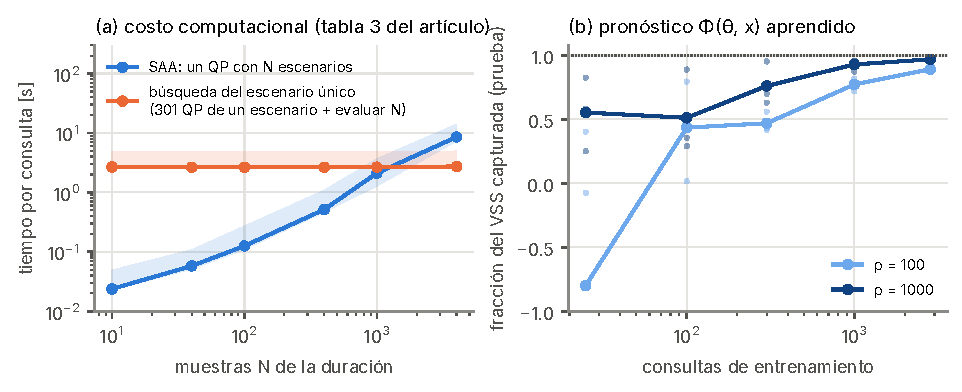
\includegraphics[width=\linewidth]{figures/fig_f9_learning.pdf}
\caption{(a) Tiempo por consulta frente al número de muestras de la duración: el SAA como un
QP (azul) y la búsqueda del escenario único (naranja); mediana y banda p10--p90 sobre 50
consultas. (b) Fracción del VSS que captura el pronóstico lineal (pérdida realizada) en las
consultas de prueba, según el número de consultas de entrenamiento (puntos: réplicas con
subconjuntos distintos).}
\label{fig:f9-learning}
\end{figure}

\begin{enumerate}
  \item \textbf{La propuesta funciona.} Un pronóstico lineal del escenario, entrenado con el
        método del artículo, captura el 89\,\% ($\rho=100$) y el 97\,\% ($\rho=1000$) del VSS fuera
        de muestra, cerca del oráculo de escenario único (93\,\% y 99.9\,\%). El techo no es 100\,\%
        porque una duración única no reproduce el SAA en todas las consultas (E3).
  \item \textbf{El contexto importa.} Un escenario fijo, sin contexto, captura entre el 31 y el
        89\,\%. El mejor margen depende del estado: del margen disponible y de la rapidez del
        calentamiento.
  \item \textbf{Hacen falta datos, y la varianza del costo realizado pesa.} El costo realizado
        tiene cola pesada (unas pocas fallas largas dominan), así que con pocas consultas el
        ajuste es ruidoso: con 25 consultas el pronóstico puede ser peor que ignorar el riesgo
        (figura~\ref{fig:f9-learning}b). La curva converge al crecer la muestra, como predice el
        teorema~2 del artículo. Integrar la duración en la pérdida (Rao--Blackwell) reduce esa
        varianza y lleva el pronóstico casi al oráculo.
  \item \textbf{Condiciones del teorema~2.} Se cumplen la continuidad de $\Phi$, la integrabilidad,
        la acotación de $Z$ y los supuestos 1--3. Dos no se cumplen en sentido estricto. (a) La
        independencia: las consultas de un mismo lazo están correlacionadas; Dias-Garcia et
        al.~\cite{diasgarcia2024} extienden el resultado a series estacionarias y ergódicas, y
        aquí la separación entre entrenamiento y prueba se hizo por realización, no por
        consulta. (b) La compacidad de $\Theta$: Nelder--Mead se usó sin cotas, aunque los
        $\theta$ ajustados quedan acotados. El teorema~4 (cota de la pérdida de aproximación)
        pide una primera etapa lineal y no aplica: aquí es cuadrática.
\end{enumerate}

\subsection{E5: lazo cerrado}\label{sec:rozas-lazo}
Los pronósticos aprendidos se pusieron dentro del lazo: en cada consulta, N2 resuelve el problema
de un escenario con $\hat\delta=\Phi(\theta,x)$ (modo \code{:scenario} de
\code{ClosedLoop.run\_loop}). Se compararon con el SAA de 40 cuantiles (el modo \code{:expected}
de F6) en los mismos 50 lazos sin fallas, con el riesgo medido por Rao--Blackwell
(tabla~\ref{tab:f9-lazo}, figura~\ref{fig:f9-closed}).

\begin{table}[H]\centering\footnotesize\setlength{\tabcolsep}{3.5pt}
\caption{Lazo cerrado, 50 realizaciones (40~kg/s, $\mu\times10^4$, $R=0.1$). $\Delta P$: diferencia
pareada con el SAA del mismo $\rho$ (IC 95\,\%). VT: variación total del caudal.}
\label{tab:f9-lazo}
\begin{tabular}{@{}llcccc@{}}
\toprule
$\rho$ & Controlador & P(1220~K $\mid$ falla) & $\Delta P$ vs SAA & pre-enfr. [K] & VT [kg/s]\\
\midrule
--- & N2 sin riesgo & 0.0311 & --- & 0.0 & 61\\
\midrule
100 & SAA (40 escenarios) & 0.0258 & --- & 1.8 & 67\\
100 & un escenario, $\Phi$ contexto completo & 0.0259 & $+0.0001\pm0.0002$ & 1.7 & 74\\
100 & un escenario, $\Phi$ variables lentas & 0.0257 & $-0.0001\pm0.0002$ & 1.8 & 72\\
100 & un escenario, $\hat D$ fijo & 0.0294 & $+0.0036\pm0.0007$ & 0.4 & 64\\
\midrule
1000 & SAA (40 escenarios) & 0.0137 & --- & 9.4 & 70\\
1000 & un escenario, $\Phi$ contexto completo & 0.0147 & $+0.0010\pm0.0003$ & 8.2 & \textbf{1694}\\
1000 & un escenario, $\Phi$ variables lentas & 0.0148 & $+0.0011\pm0.0004$ & 8.2 & 84\\
1000 & un escenario, $\hat D$ fijo & 0.0178 & $+0.0041\pm0.0008$ & 5.6 & 84\\
\bottomrule
\end{tabular}
\end{table}

\begin{figure}[H]\centering
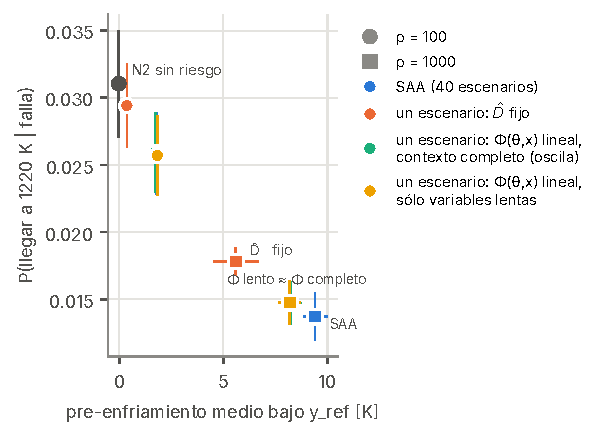
\includegraphics[width=0.75\linewidth]{figures/fig_f9_closed.pdf}
\caption{Riesgo frente a pre-enfriamiento en lazo cerrado (50 realizaciones, IC 95\,\%). Círculos:
$\rho=100$; cuadrados: $\rho=1000$. Los dos pronósticos contextuales coinciden en este plano; el
de contexto completo oscila (tabla~\ref{tab:f9-lazo}).}
\label{fig:f9-closed}
\end{figure}

\begin{enumerate}
  \item \textbf{Con $\rho=100$, el MPC de un escenario es el SAA.} Mismo riesgo, mismo
        pre-enfriamiento, misma suavidad, resolviendo un QP de un escenario en vez de uno de 40.
  \item \textbf{Con $\rho=1000$, el pronóstico con todo el contexto hace oscilar el lazo.} El riesgo
        y el pre-enfriamiento quedan cerca del SAA, pero el caudal oscila (VT de 1694 frente a 70
        kg/s). El pronóstico baja el margen $\hat\delta$ unos 10~K por desviación estándar del
        margen \emph{actual}. Entonces el techo de la PCT, $1220-\hat\delta$, se mueve en contra de
        la PCT con ganancia $\approx1.6>1$: si la PCT baja, el pronóstico permite calentar; si sube,
        exige enfriar. Es una realimentación inestable de periodo~2.
  \item \textbf{La causa es que el contexto es endógeno.} El artículo supone que el contexto $x$
        es exógeno (datos i.i.d.): la decisión no cambia el contexto siguiente. En un MPC sí lo
        cambia. Al reajustar $\Phi$ sólo con las variables lentas (la fuga y el calentamiento a 46,
        150 y 400~s), que el caudal casi no mueve de una consulta a la siguiente, la oscilación
        desaparece (VT 84~kg/s) y el riesgo y el pre-enfriamiento no cambian. Fuera de muestra, ese
        pronóstico sigue capturando el 91.7\,\% ($\rho=100$) y el 99.7\,\% ($\rho=1000$) del VSS.
  \item \textbf{Queda una brecha pequeña con $\rho=1000$} ($\Delta P=+0.001$, 1.2~K menos de
        pre-enfriamiento). No es una pérdida de eficiencia: el punto está sobre la misma frontera
        riesgo--pre-enfriamiento (sección~\ref{sec:riesgo-formulaciones}). Equivale a un $\rho$ algo
        menor.
  \item \textbf{Un escenario fijo, sin contexto, protege menos} que el SAA con el mismo $\rho$:
        $\Delta P=+0.004$.
\end{enumerate}

\takeaway{\textbf{Para recordar.} El SMDFR cumple las condiciones del teorema~1 en la pérdida
esperada (caso i) y, escrita por paso, en las fallas parciales (caso ii, lema~1~iii); la
unicidad la da la supresión de movimiento $R$. El escenario del teorema reproduce la decisión
estocástica en todas las formulaciones, pero no es un evento físico. Una sola falla bien
elegida recupera el 94--99.5\,\% del VSS y el pronóstico puntual no recupera nada. La propuesta
de Rozas funciona: un pronóstico lineal del escenario, aprendido con el método del artículo,
captura el 89--97\,\% del VSS fuera de muestra y, en lazo cerrado, reproduce el riesgo del SAA,
siempre que el pronóstico dependa sólo de variables que la decisión no mueve de una consulta a
la siguiente. Si depende del margen actual, el lazo oscila: el artículo supone un contexto
exógeno y en un MPC no lo es.}
